\documentclass[oneside]{book}
\usepackage[utf8x]{inputenc}    
\usepackage[T1]{fontenc}
\usepackage[francais]{babel}     
\usepackage{listings}
\usepackage{graphicx}
\usepackage{courier}
\pagenumbering{arabic}
\title{Travaux Pratiques - Probabilités}

\author{Dylan \bsc{TROLES} \& Hugo \bsc{POULIQUEN}}

\date{4 mai 2016}

\begin{document}

\maketitle

\chapter{Génération de nombres pseudo-aléatoires}
\section{Approche fréquentielle des probabilités}
\subsection{Le lancer de 5 dés}
Une épreuve consiste à lancer 5 dés et à considérer la somme amenée à chaque lancer.
Construire un programme qui donne : 
\begin{enumerate}
	\item Les valeurs de la somme, le nombre de sorties possibles pour chaque valeur, et la fréquence de chaque sortie.
	\item Un tableau et un graphique donnant les fréquences de chaque sortie.
\end{enumerate}
Pour cet exercice, nous avons fait un script python. Pour pouvoir lancer ce script, il est nécessaire d'installer la librairie matplotlib.
\lstinputlisting[basicstyle=\ttfamily,numbers=left,caption=Lancer\_de\_5\_des.py,language=Python]{../lancer_de_5_des.py}
Voici le résultat généré par le script : 
\begin{lstlisting}[frame=single]
$ python3 lancer_de_5_des.py 

Traitement pour : 5 des comportant 6 faces de 1 a 6
Nombre de sommes possibles : 25

-> Lancement des des...
Somme des des lances : 21
\end{lstlisting}
Tableau du nombre de combinaisons possibles pour chaque somme :
\begin{lstlisting}[frame=single]
5 : 1
6 : 5
7 : 15
8 : 35
9 : 70
10 : 126
11 : 205
12 : 305
13 : 420
14 : 540
15 : 651
16 : 735
17 : 780
18 : 780
19 : 735
20 : 651
21 : 540
22 : 420
23 : 305
24 : 205
25 : 126
26 : 70
27 : 35
28 : 15
29 : 5
30 : 1
\end{lstlisting}
Tableau des frequences de chaque somme :
\begin{lstlisting}[frame=single]
5 : 0.01286008230452675
6 : 0.06430041152263374
7 : 0.19290123456790123
8 : 0.45010288065843623
9 : 0.9002057613168725
10 : 1.6203703703703702
11 : 2.6363168724279835
12 : 3.9223251028806585
13 : 5.401234567901234
14 : 6.944444444444445
15 : 8.371913580246913
16 : 9.452160493827162
17 : 10.030864197530864
18 : 10.030864197530864
19 : 9.452160493827162
20 : 8.371913580246913
21 : 6.944444444444445
22 : 5.401234567901234
23 : 3.9223251028806585
24 : 2.6363168724279835
25 : 1.6203703703703702
26 : 0.9002057613168725
27 : 0.45010288065843623
28 : 0.19290123456790123
29 : 0.06430041152263374
30 : 0.01286008230452675
\end{lstlisting}
Voici le graphe généré : 
\begin{figure}[h!]
	\centering
	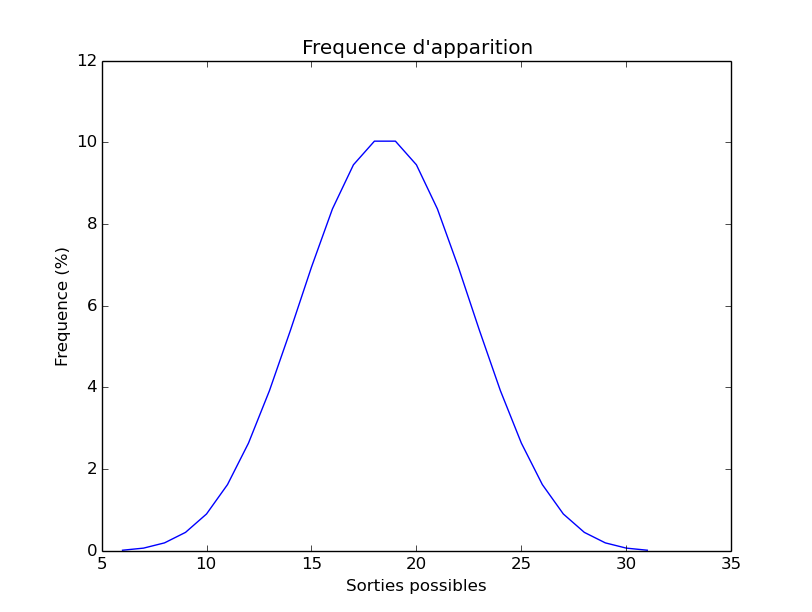
\includegraphics[width=\textwidth]{lancer_de_5_des.png}
	\caption{Sorties possibles en lançant 5 dés différents en 1 fois}
\end{figure}
\section{Nombres pseudo aléatoires}
\textbf{Exercice 1 :}
\begin{enumerate}
	\item Votre machine a une fonction RAND qui vous fournit de manière aléatoire un nombre de [0,1[. Donner un algorithme utilisant la fonction RAND fournissant un nombre entier entre 1 et N.
	\item Pouvez-vous être satisfait de la fonction fournie par le constructeur ?
\end{enumerate}
\lstinputlisting[basicstyle=\ttfamily,numbers=left,caption=Nombre\_pseudo\-aleatoires\_exo1.py,language=Python]{../Nombre_pseudo-aleatoires_exo1.py}
\textbf{Réponse :} 
Au vu du graphe, l'aléatoire de la fonction random.randrange donnée par le constructeur n'est pas satisfaisant. Chaque barre devrait avoir une probabilité de $\frac{1}{N}$ car nous sommes dans l'ensemble \{1, ..., N\}. Dans notre exemple, N = 10. Pour chaque barre, $\frac{1}{N}$ devrait donc être égale à 0,10 .

Prenons la première barre, on remarque que la valeur 1 est sortie 918 fois Calculons sa probabilité : $\frac{918}{10000}$ = 0.0918

Prenons la dernière barre, on remarque que la valeur 10 est sortie 1736 fois Calculons sa probabilité : $\frac{1736}{10000}$ = 0.1736

Les probabilités d'apparitions de chaque valeur ne respecte donc pas 0.10. En conclusion, la fonction random.randrange n'est pas aléatoire et pour notre exemple, la valeur 10 apparait le plus souvent.
\newpage
Voici le graphe généré par le script précédent : 
\begin{figure}[h!]
	\centering
	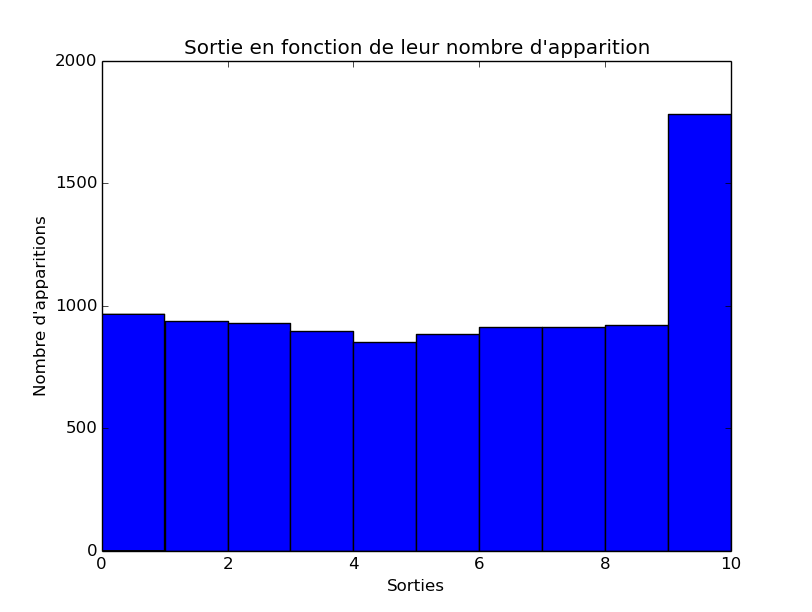
\includegraphics[width=\textwidth]{Nombre_pseudo-aleatoires_exo1.png}
	\caption{Sortie en fonction de leur nombre d'apparition}
	\label{fig:cc40}
\end{figure}
\newline
\textbf{Exercice 2 :}
Voici un programme écrit dans le langage algorithmique TestAlgo.
Ce petit programme peut être amélioré.
\begin{lstlisting}[frame=single]
algo Nombres aleatoires
var
  entier i,z;
principal
  debut
	  i:=1
		tantque (i<=100)
		  z:=arrondi(3*aleatoire());
			afficher(z)
			i:=i+1;
		fintantque
	fin
\end{lstlisting} 
\newpage Que réalise ce programme ? Qu'en pensez-vous ? \newline 
\begin{figure}[h!]
	\centering
	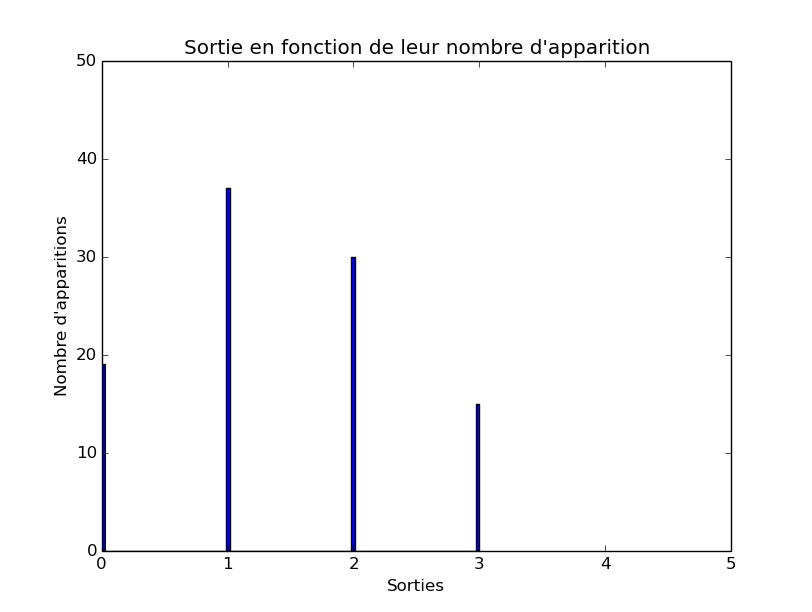
\includegraphics[width=\textwidth]{Nombre_pseudo-aleatoires_exo2.png}
	\caption{Sortie en fonction de leur nombre d'apparition}
	\label{fig:cc40}
\end{figure}
\textbf{Réponse :} \newline
Ce programme donne un nombre entier entre 0 et 3.

Au vu du graphe nous pensons que cet algorithme se rapproche d'un algorithme aléatoire mais n'en est pas un. Pour le prouver calculons la probabilité théorique de chaque valeur :\newline \newline $\frac{1}{N+1}$ = 0.25 avec N = 3 \newline \newline
Voici les fréquences observées à partir du graphe dans l'expérimentation \newline
0 : 0,15 \newline 1 : 0,32 \newline 2 : 0,33 \newline 3 : 0,20 \newline

Cette fois, les probabilités obtenues se rapprochent un peu plus de la probabilité théorique. L'aléatoire n'est toujours pas uniforme.
\section{Génération de nombres aléatoires}
\subsection{Générateurs congruentiels linéaires}
\textbf{Exercice 3 :}
Donner la suite des nombres aléatoires et en rechercher les périodes pour : 
\begin{enumerate}
	\item b = 3, $X_0$ = 7, a = 5, N = 16 
	\begin{lstlisting}[frame=single]
	-- b = 3, X0 = 7, a = 5, N = 16--
n  = 0 1 2 3 4  5  6 7  8  9 10 11 12 13 14 15 16 
Xn = 7 6 1 8 11 10 5 12 15 14 9 0  3  2  13 4  7 
La periode est de : 16
\end{lstlisting}
	\item b = 6, $X_0$ = 7, a = 5, N = 16 
	\begin{lstlisting}[frame=single]
	-- b = 6, X0 = 7, a = 5, N = 16--
n  = 0 1 2 3 4  5 6  7  8 9  10 11 12 13 14 15 16 
Xn = 7 9 3 5 15 1 11 13 7 9  3  5  15 1  11 13 7 
La periode est de : 8

	\end{lstlisting}
	\item b = 0, $X_0$ = 1, a = 2, N = 17 
	\begin{lstlisting}[frame=single]
	-- b = 0, X0 = 1, a = 2, N = 17--
n  = 0 1 2 3 4  5  6  7 8 9 10 11 12 13 14 15 16 17 
Xn = 1 2 4 8 16 15 13 9 1 2 4  8  16 15 13 9  1  2 
La periode est de : 8
	\end{lstlisting}
	\item b = 6, $X_0$ = 1, a = 2, N = 17 
	\begin{lstlisting}[frame=single]
	-- b = 6, X0 = 1, a = 2, N = 17--
n  = 0 1 2 3  4 5  6 7 8 9 10 11 12 13 14 15 16 17 
Xn = 1 8 5 16 4 14 0 6 1 8 5  16 4  14 0  6  1  8 
La periode est de : 8

	\end{lstlisting}
	\item b = 0, $X_0$ = 3, a = 13, N = $2^7$ 
	\begin{lstlisting}[frame=single]
	-- b = 0, X0 = 3, a = 13, N = 128--
La suite est trop importante pour etre affichee

La periode est de : 32

	\end{lstlisting}
	\item b = 0, $X_0$ = 4567, a = 9749, N = $2^{17}$
	\begin{lstlisting}[frame=single]
	-- b = 0, X0 = 4567, a = 9749, N = 131072--
La suite est trop importante pour etre affichee

La periode est de : 32768
    \end{lstlisting}
\end{enumerate}
Ces résultats sont issus du script suivant :
\lstinputlisting[basicstyle=\ttfamily,numbers=left,caption=Nombre\_pseudo-aleatoires\_exo3.py,language=Python]{../Nombre_pseudo-aleatoires_exo3.py}
\newpage
\textbf{Exercice 4 :}
\begin{enumerate}
	\item Écrire une fonction Scilab qui pour argument de sortie une suite ($U_{n}$)$_{n}$ $\in$ $\mathbf{N}$ de réels compris entre 0 et 1, générée par un générateur congruentiel linéaires, et pour argument d'entrée $X_0$, a, b et N, les paramètres usuels d'un tel générateur.\newline
\textbf{Réponse :} 
\lstinputlisting[basicstyle=\ttfamily,numbers=left,caption=Exercice4.sce,language=Scilab]{../Exercice4.sce}
	\item En utilisant la fonction écrite en Scilab, étudiez les générateurs qui suivent : on regardera, en particulier, et si c'est possible, la période.
	\begin{itemize}
		\item Pour a = 25, b = 16 et N = 256 = $2^8$ et pour $X_0$ successifs : $X_0$ = 12; $X_0$ = 11 ; $X_0$ = 0
		\item \textbf{Turbo-Pascal} a = 129, b = 907633385 et N = $2^{32}$
		\item \textbf{Unix} a = 1103515245, b = 12345 et N = $2^{32}$
		\item \textbf{Matlab} a = 19807, b = 0 et N = $2^{31}$-1
	\end{itemize}
\end{enumerate}
\section{Autres méthodes}
\subsection{Méthode de VON NEUMANN}
Comment fonctionne cette méthode ?
\begin{itemize}
	\item On se donne un nombre A de N chiffres
	\item On l'élève au carré
	\item On choisit comme nombre suivant le nombre de N chiffres formé par la tranche du milieu du carré obtenu
	\item On divise ensuite par $10^N$
\end{itemize}
\begin{enumerate}
	\item Montrer que l'on obtient bien une suite de nombres compris entre 0 et 1 (1 exclu)\newline
	\textbf{Réponse :} A est un nombre de N chiffres. \newline
	10$^{N-1}$ $\le$ A < 10$^N$\newline
	On élève au carré : 10$^{2N-2}$ $\le$ A$^2$ < 10$^{2N}$\newline
	B est le nouveau nombre formé par la tranche du milieu du carré obtenu :\newline
	10$^{N-1}$ $\le$ B < 10$^N$\newline
	On divise par 10$^N$ : 0,1 $\le$ $\frac{B}{10^N}$  < 1
	\item Donner un algorithme fournissant ces nombres \newline
	\textbf{Réponse :} 
	\lstinputlisting[basicstyle=\ttfamily,numbers=left,caption=VonNeumann.py,language=Python]{../VonNeumann.py}
	\item Faire une étude pour N = 4, et A = 5678 \newline
	\textbf{Réponse :} \begin{lstlisting}[frame=single]
	A=5678 
	N=4 
	Carre de A=32239684 
	Tranche=2396 
	Resultat=0.2396 \end{lstlisting}
	\item Faire une étude pour N = 6, et A de votre choix \newline
	\textbf{Réponse :} \begin{lstlisting}[frame=single]
	A=123456
 	N=6
	Carre de A=15241383936
	Tranche=241383
	Resultat=0.241383
	\end{lstlisting}
	\item Que penser de cette méthode ? \newline
	\textbf{Réponse :} \newline
	Pour 100 lancés, on obtient les résultats de la figure suivante. Ces résultats montrent que l'aléatoire de VonNeumann n'uniformise pas les numéros de sortie. Si l'on compare avec la fonction random de Python (cf Ex1), VonNeumann est nettement plus aléatoire. La différence entre les apparitions de chaque valeur est moins importante que dans l'analyse de l'exercice 1.\newline
	Cette méthode est plus aléatoire que la fonction random de Python, mais n'est pas uniforme car toutes les valeurs n'ont pas le même nombre d'apparitions.
	\begin{figure}[h!]
		\centering
			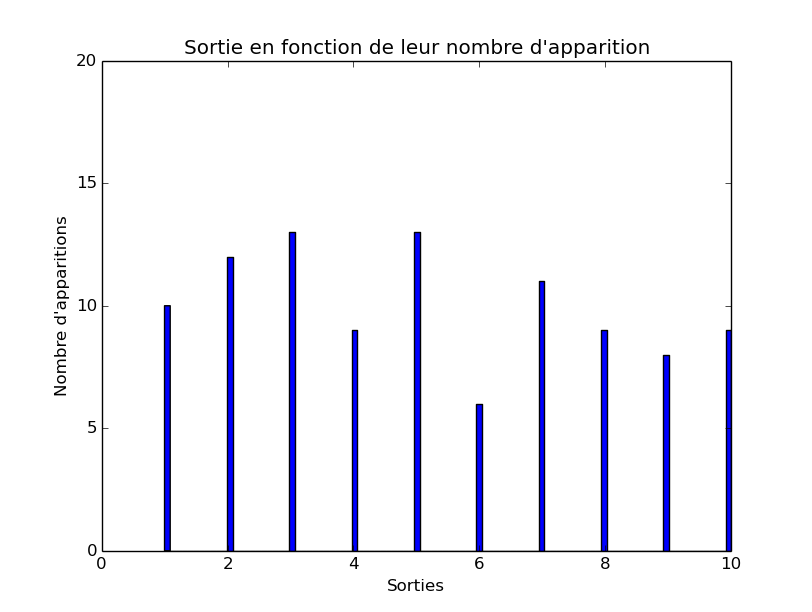
\includegraphics[width=\textwidth]{VonNeumann.png}
		\caption{Sortie en fonction de leur nombre d'apparition}
\end{figure}
\end{enumerate}
\end{document}